\section{Experiments}
%In this section, we present the experiments of LPAF for language model compression. We compare with state-of-the-art compression methods and perform detailed analysis of the results to provide guidance under different resource budgets.
\subsection{Experimental Setup}
\subsubsection{Datasets} 
%\subsection{Datasets}
We evaluate our approach on the following tasks: Corpus of Linguistic Acceptability~(\textbf{CoLA}) which judges if a sentence is grammatically correct, Stanford Sentiment Treebank~(\textbf{SST-2})~\cite{sst2} which is 
a binary sentiment classification task,
Quora Question Pairs~(\textbf{QQP}) which is a paraphrase similarity matching task,
Multi-Genre Natural Language Inference~(\textbf{MNLI})~\cite{mnli} and \textbf{QNLI}, which are two NLI tasks, 
and finally, \textbf{SQuAD v1.1}~\cite{qnliandsquad} and \textbf{SQuAD v2.0}~\cite{squad2} which are two extractive 
question answering tasks. All tasks use accuracy as the evaluation metric, while CoLA uses Matthew's Correlation and SQuAD uses the F1 score.

Following previous work~\cite{pkd}, we evaluate under a task-specific setting, i.e., we utilize no external corpus but only assume access to the training data of each task.



\subsubsection{Baselines} We compare against compression methods that lead to \textbf{\textit{perceivable reduction in model size and computation}}, i.e., knowledge distillation and matrix factorization:
\textbf{DistilBERT}~\cite{distilbert}, \textbf{PD-BERT}~\cite{pdbert}, and \textbf{TinyBERT}~\cite{tinybert} are  task-agnostic distillation methods involving a pre-training compression stage using unlabeled corpus followed by task-specific fine-tuning; \textbf{BERT$_\text{Truncated}$} directly fine-tunes a truncated BERT model; \textbf{KD} uses vanilla logits-based knowledge distillation~\cite{kd}; \textbf{PKD}~\cite{pkd} introduces patient distillation for intermediate feature matching; 
%  \textbf{RAIL-KD}~\cite{rail} randomizes the layer mapping which is fixed in PKD; 
\textbf{Theseus}~\cite{theseus} proposed a new genre of model compression by progressive module replacing; \textbf{CKD}~\cite{CKD} utilizes a novel KD objective to transfer the contextual knowledge via word relation and layer transforming relation; \textbf{MetaDistil}~\cite{metadistil} introduces meta-learning for training the teacher to better transfer knowledge to the student; \textbf{SVD}$_{\text{Pre}}$/\textbf{SVD}$_{\text{Ft}}$~\cite{svd} applies standard singular value decomposition on pre-trained/densely fine-tuned model and re-trains the decomposed model. We report the results of full-version LPAF as well as its three ablated versions that remove each of the three procedures in Algorithm \ref{alg:lpaf}. Comparisons with architecture-dependent structured pruning~\cite{l0} are deferred to Appendix C. 
%  We obtain the results of all baselines by running their official implementations.

\subsubsection{Implementation Details}
In the main experiment, we adopt SMvP as the default choice of the first-order pruning method due to its training efficiency compared to CAP. The results of LPAF with CAP can be found in Appendix C. We tune the pruning hyper-parameter $\tau$ such that $T_{sparse}$ obtained by SMvP retains at least 97\% performance of densely fine-tuned BERT. We search $p_{init}$ in \{0.7, 0.5, 0.3\} and decay it to zero after half of the total training steps. We discuss the influence of different $p_{init}$ in \secref{sec:analysis}. During training, we
fix the batch size to 32 to reduce the search space. The max input length is set to 384 for SQuAD and 128 for other tasks. We use the AdamW~\cite{adamw} optimizer and search learning rate in \{2e-5,3e-5\}. The training epochs are set to 6. We report the results on the test set for SQuAD and the development set for others.
%All experiments are conducted on an RTX 2080Ti GPU with 12GB RAM.

\subsubsection{Compression Setting}

We compress a 86M parameter  BERT-base model into compact ones of various sizes. 
We refer to BERT-base compressed by  LPAF with preserved rank $k$ as LPAF-$k$. We select $k$ from \{120,100,80,60,40\}, which corresponds to \{22\%,19\%,15\%,12\%,8\%\} of original parameters. In addition, we also report FLOPs to measure the computation cost based on the number of floating-point operations for processing one sample, i.e., batch size = 1.

All baselines except for SVD achieve different compression ratios by 
varying the number 
of encoder layers, hence comparison under the same model size is infeasible. 
We therefore set the number of layers in these baseline models to \{3, 2, 1\}, 
which corresponds to \{25\%, 16\%, 8\%\} of BERT's parameters. 
This makes their model sizes and FLOPs roughly equal to those of SVD/LPAF-120/80/40. 
SQuAD needs higher FLOPs than other tasks given the same rank $k$ due to its longer input length. See \tabref{table:stats} for details.

% \begin{table}[th]
% 	\scriptsize
% 	\centering
% 	\begin{tabular}{l|cc|cc}
% 		\toprule
% 		Task& \multicolumn{2}{c|}{Others} & \multicolumn{2}{c}{SQuAD v1.1} \\
% 		\midrule
% 		Metric & \% of Param.           & FLOPs               & \% of Param.      & FLOPs        \\
% 		\midrule
% 		BERT-base & 100               & 7.4G                & 100        & 35.4G        \\
% 		$T_{sparse}$ & 100               & 7.4G                & 100        & 35.4G        \\
% 		\midrule
% 		LPAF-120   & 22       & 1.9G          & 22  & 10.3G  \\
% 		LPAF-100   & 19      & 1.6G          & 19  & 9.1G   \\
% 		LPAF-80    & 15       & 1.3G          & 15  & 7.9G   \\
% 		LPAF-60    & 12        & 1.0G         & 12  & 6.6G   \\
% 		LPAF-40    & 8        & 0.7G        & 8  & 5.3G \\ 
% 		\bottomrule
% 	\end{tabular}
% 	\caption{Percentage of parameters and FLOPs. $T_{sparse}$ has identical parameters and FLOPs as BERT-base because it only sets certain weights to zero without actually eliminating them from the computation.}
% 	\label{table:stats}
% \end{table}

\begin{table}[th]
	\scriptsize
	\centering
	\begin{tabular}{|l|cl|cc|}
%		\toprule
\hline
		Metric       & \multicolumn{2}{c|}{\% of Parameters} & \multicolumn{2}{c|}{FLOPs} \\ 
%		\midrule
\hline
		Task         & \multicolumn{2}{c|}{All}          & Others    & SQuAD v1.1/v2.0    \\ 
%		\midrule
\hline
		BERT-base    & \multicolumn{2}{c|}{100}          & 7.4G      & 35.4G         \\
		$T_{sparse}$ & \multicolumn{2}{c|}{100}          & 7.4G      & 35.4G         \\ 
%		\midrule
\hline
		LPAF-120     & \multicolumn{2}{c|}{22}           & 1.9G      & 10.3G         \\
		LPAF-100     & \multicolumn{2}{c|}{19}           & 1.6G      & 9.1G          \\
		LPAF-80      & \multicolumn{2}{c|}{15}           & 1.3G      & 7.9G          \\
		LPAF-60      & \multicolumn{2}{c|}{12}           & 1.0G      & 6.6G          \\
		LPAF-40      & \multicolumn{2}{c|}{8}            & 0.7G      & 5.3G          \\ 
%		\bottomrule
\hline
	\end{tabular}
	\caption{Percentage of parameters and FLOPs. $T_{sparse}$ has identical parameters and FLOPs as BERT-base because the pruned weights still participate in computation and storage.}
	\label{table:stats}
\end{table}
\begin{table*}[thb!]
	\centering
	\scriptsize
	\begin{tabular}{|l|cccccc|}
		%		\toprule
		\hline
		Task &CoLA~(8K) & SST-2~(67K)                                                  & QQP~(364K)                                                    & QNLI~(105K)                                                & MNLI-m/mm~(393K)                                                 & SQuAD v1.1/v2.0~(88/131K)         \\
		%		\midrule
		\hline
		\% of \#Parameters~$\downarrow$   &25\% ~16\%  ~~8\%            &25\% ~16\%  ~~8\%             &25\% ~16\%  ~~8\%            &25\% ~16\%  ~~8\%            &25\% ~~~~~~~~16\%  ~~~~~~~~~8\%     &25\% ~~~~~~~~16\%  ~~~~~~~~8\%       \\
		\hline
		\multicolumn{7}{|c|}{\textit{\textbf{Knowledge Distillation}}}   \\
		\hline
		DistilBERT  &32.1~ 21.1~ 10.1    & 88.9 ~86.4 ~83.0          & 89.4~ 88.0~ 82.4          & 83.8~ 81.6~ 64.9          & 76.4/76.4 ~71.6/70.9 ~59.8/58.6          & 78.0/62.5~ 66.5/56.2 ~28.5/47.6       \\
		PD-BERT     &33.1~ 24.8~ 15.8   & 88.2~ 87.5~ 82.7          & 89.8 ~88.9 ~82.9          & 86.1~ 83.4~ 65.9          & 78.6/78.3 ~75.9/75.9 ~66.0/65.9          & 77.0/64.5 ~45.2/55.4~ 22.8/47.3       \\
		TinyBERT    &33.3~ 21.3 ~14.9   & 89.8 ~88.0 ~82.6          & 90.0~ 88.7~ 83.2          & 87.7 ~84.5~ 63.1          & 80.6/80.5~ 77.1/77.7~ 65.6/66.2          & 58.0/64.9 ~38.1/57.6 ~15.4/48.2     \\
		%		\midrule
		%		\hline
		%\multicolumn{6}{c}{\textit{Task-specific Distillation}}   \\
		%\midrule
		BERT$_{\text{Truncated}}$  &19.7~ 18.9~ 13.2 & 87.7 ~85.6 ~79.6          & 88.0~ 86.9 ~82.2          & 83.0 ~78.7 ~60.3          & 75.7/73.2~ 73.1/72.3~ 60.6/60.3          & 54.8/58.3~ 31.4/50.1~ 17.1/47.9        \\
		KD    &21.8~ 18.7~ 13.2  & 88.5~ 86.5 ~82.0           & 88.8~ 87.2 ~82.3          & 83.6 ~78.6~ 59.8          & 76.1/73.5 ~73.3/72.6~ 61.3/61.2          & 62.5/60.6 ~32.3/52.2~ 17.0/49.4       \\
		PKD  &22.0~ 19.1~ 14.1   & 88.1~ 87.2 ~82.0          & 88.5~ 87.5 ~82.3          & 82.7~ 78.0~ 59.8          & 75.8/75.6 ~73.0/72.3~ 61.3/61.2          &60.5/60.8~ 31.5/52.5~ 17.0/49.9                                             \\
		Theseus&17.9~ 17.6~ 13.6  & 88.5~ 86.1~ 79.6          & 89.0 ~86.0 ~82.2          & 85.0 ~80.3~ 60.3          & 76.3/76.4~ 73.4/73.6 ~60.6/60.3          &72.7/60.7~ 63.2/55.0~ 26.2/48.0                                            \\
		% RAIL-KD~\cite{rail}     &   & 88.8~ 86.8~ 83.9          &\underline{90.2} ~88.6 ~\underline{83.3}          &85.7 ~81.2~ 65.7          &78.8/78.8 ~73.5/74.0 ~62.1/61.4          &78.7~ 69.5~ 32.1                                                      \\
		CKD   &40.1~ 32.9~ 17.3   & 89.8 ~88.7~ 84.1          & 90.1~ 88.9~ 82.9          & 87.0~ 84.9 ~67.6          & 79.1/78.9 ~76.8/76.8~ 66.4/66.7          &78.9/65.2~ 69.1/60.1~ 33.1/51.6                            \\
		MetaDistil  &33.6~ 24.3~ 13.7    & 88.9 ~87.0~ 82.7          & 88.9~ 86.9~ 82.1          & 86.8~ 84.9 ~67.5          & 79.2/79.7 ~76.7/77.0~ 66.4/66.7          &78.8/65.0~ 69.0/59.8~ 32.4/50.4                           \\
		\hline
		\multicolumn{7}{|c|}{\textit{\textbf{Matrix Factorization}}}   \\
		\hline
		SVD$_{\text{Pre}}$  &22.2~ 16.0~ 12.7    & 86.6 ~84.9~ 84.2         & 88.2 ~86.7~ 82.4          & 85.3 ~81.6~ 68.9          & 78.3/79.3~ 76.0/76.7~ 70.8/71.3          & 82.7/67.5~ 79.4/63.5~ 45.2/48.5      \\
		SVD$_{\text{Ft}}$  &26.6~ 18.0~ 12.2    & 88.9 ~85.3~ 84.5         & 90.0 ~87.9~ 83.1          & 86.1 ~83.8~ 67.6          & 79.6/80.2~ 76.6/76.7~ 71.6/72.2          & 85.5/74.6~ 81.1/72.1~ 51.3/62.3     \\
		LPAF~(ours)   &\textbf{48.5~ 42.8~ 34.3}     & \textbf{90.7~ 89.7~ 88.5} & \textbf{90.4}~ \textbf{90.1}~ \textbf{89.0} & \textbf{89.2~ 88.6~ 85.7} & \textbf{82.2/82.9}~ \textbf{81.4/81.9}~ \textbf{79.2/80.1} & \textbf{87.2/77.2 ~85.7/75.1 ~82.0/71.5} \\
		~~-w/o Step-1    &32.9~ 18.2~ 16.0    &89.9~ 88.4 ~86.0 &90.3~ 89.7~ 86.9 &87.8~ 84.8~ 73.6 &81.6/82.4~ 79.2/79.8~ 72.2/72.0 &86.5/75.6~ 83.5/72.7~ 71.0/63.9  \\
		~~-w/o Step-2     &48.0~ 41.0~ 32.6   &89.2~ 88.8~ 87.3 &90.2~ 90.0~ 88.7 &89.0~ 87.9~ 85.0 &82.0/82.7~ 81.2/81.8~ 79.0/80.0 &87.0/76.8~ 85.5/74.9~ 81.4/69.6 \\
		~~-w/o Step-3    &48.2~ 42.2~ 32.6     &89.5~ 88.8~ 87.9 &90.3~ 89.9~ 88.8 &88.9~ 88.1~ 85.0 &81.0/81.7~ 80.6/81.3~ 78.3/78.9 &86.8/76.6~ 85.4/74.9~ 81.3/70.7\\
		%		\bottomrule
		\hline
	\end{tabular}
	\caption{Experimental results~(average of 3 runs) of different compression methods applied on BERT-base. The best results are \textbf{bolded}. The numbers in the parenthesis are training data sizes for each task.}
	\label{table:all}
\end{table*}
%\begin{table*}[thb!]
%	\centering
%	\scriptsize
%	\begin{tabular}{|l|cccccc|}
%		%		\toprule
%		\hline
%		Task  & SST-2~(67K)                                                  & QQP~(364K)                                                    & QNLI~(105K)                                                   & MNLI-m/mm~(393K)                                                   & SQuAD v1.1~(88K)                                & SQuAD v2.0~(131K)             \\
%		%		\midrule
%		\hline
%		\% of \#Parameters~$\downarrow$  &25\% ~16\%  ~~8\%            &25\% ~16\%  ~~8\%             &25\% ~16\%  ~~8\%            &25\% ~~~~~~~~~	~16\%  ~~~~~~~~~~8\%            &25\% ~16\%  ~~8\%     &25\% ~16\%  ~8\%       \\
%			 			\hline
%		 \multicolumn{7}{|c|}{\textit{Knowledge Distillation}}   \\
%		 			\hline
%		DistilBERT     & 88.9 ~86.4 ~83.0          & 89.4~ 88.0~ 82.4          & 83.8~ 81.6~ 64.9          & 76.4/76.4 ~71.6/70.9 ~59.8/58.6          & 78.0~ 66.5 ~28.5   &62.5~ 56.2~ 47.6       \\
%		PD-BERT        & 88.2~ 87.5~ 82.7          & 89.8 ~88.9 ~82.9          & 86.1~ 83.4~ 65.9          & 78.6/78.3 ~75.9/75.9 ~66.0/65.9          & 77.0 ~45.2~ 22.8 &64.5~ 55.4~ 47.3         \\
%		TinyBERT       & 89.8 ~88.0 ~82.6          & 90.0~ 88.7~ 83.2          & 87.7 ~84.5~ 63.1          & 80.6/80.5~ 77.1/77.7~ 65.6/66.2          & 58.0 ~38.1 ~15.4    &64.9~ 57.6~ 48.2      \\
%		%		\midrule
%%		\hline
%		%\multicolumn{6}{c}{\textit{Task-specific Distillation}}   \\
%		%\midrule
%		BERT$_{\text{Truncated}}$  & 87.7 ~85.6 ~79.6          & 88.0~ 86.9 ~82.2          & 83.0 ~78.7 ~60.3          & 75.7/73.2~ 73.1/72.3~ 60.6/60.3          & 54.8~ 31.4~ 17.1   &58.3~ 50.1~ 47.9       \\
%		KD      & 88.5~ 86.5 ~82.0           & 88.8~ 87.2 ~82.3          & 83.6 ~78.6~ 59.8          & 76.1/73.5 ~73.3/72.6~ 61.3/61.2          & 62.5 ~32.3~ 17.0    &60.6~ 52.2~ 49.4      \\
%		PKD    & 88.1~ 87.2 ~82.0          & 88.5~ 87.5 ~82.3          & 82.7~ 78.0~ 59.8          & 75.8/75.6 ~73.0/72.3~ 61.3/61.2          &60.5~ 31.5~ 17.0       &60.8~ 52.5~ 49.9                                               \\
%		Theseus  & 88.5~ 86.1~ 79.6          & 89.0 ~86.0 ~82.2          & 85.0 ~80.3~ 60.3          & 76.3/76.4~ 73.4/73.6 ~60.6/60.3          &72.7~ 63.2~ 26.2                &60.7~ 55.0~ 48.0                                      \\
%		% RAIL-KD~\cite{rail}     &   & 88.8~ 86.8~ 83.9          &\underline{90.2} ~88.6 ~\underline{83.3}          &85.7 ~81.2~ 65.7          &78.8/78.8 ~73.5/74.0 ~62.1/61.4          &78.7~ 69.5~ 32.1                                                      \\
%		CKD     & 89.8 ~88.7~ 84.1          & 90.1~ 88.9~ 82.9          & 87.0~ 84.9 ~67.6          & 79.1/78.9 ~76.8/76.8~ 66.4/66.7          &78.9~ 69.1~ 33.1           &65.2~ 60.1~ 51.6                                           \\
%		MetaDistil     & 88.9 ~87.0~ 82.7          & 88.9~ 86.9~ 82.1          & 86.8~ 84.9 ~67.5          & 79.2/79.7 ~76.7/77.0~ 66.4/66.7          &78.8~ 69.0~ 32.4          &65.0~ 59.8~ 50.4                                            \\
%			 			\hline
%\multicolumn{7}{|c|}{\textit{Matrix Factorization}}   \\
%\hline
%		SVD$_{\text{Pre}}$     & 86.6 ~84.9~ 84.2         & 88.2 ~86.7~ 82.4          & 85.3 ~81.6~ 68.9          & 78.3/79.3~ 76.0/76.7~ 70.8/71.3          & 82.7~ 79.4~ 45.2    &67.5 ~63.5~ 48.5      \\
%		SVD$_{\text{Ft}}$     & 88.9 ~85.3~ 84.5         & 90.0 ~87.9~ 83.1          & 86.1 ~83.8~ 67.6          & 79.6/80.2~ 76.6/76.7~ 71.6/72.2          & 85.5~ 81.1~ 51.3     &74.6~ 72.1~ 62.3     \\
%		LPAF~(ours)        & \textbf{90.7~ 89.7~ 88.5} & \textbf{90.4}~ \textbf{90.1}~ \textbf{89.0} & \textbf{89.2~ 88.6~ 85.7} & \textbf{82.2/82.9}~ \textbf{81.4/81.9}~ \textbf{79.2/80.1} & \textbf{87.2 ~85.7 ~82.0} & \textbf{77.2}~ \textbf{75.1}~ \textbf{71.5}\\
%		~-~w/o low-rank pruning        &89.9~ 88.4 ~86.0 &90.3~ 89.7~ 86.9 &87.8~ 84.8~ 73.6 &81.6/82.4~ 79.2/79.8~ 72.2/72.0 &86.5~ 83.5~ 71.0 &75.6~ 72.7~ 63.9 \\
%		~-~w/o sparsity-aware SVD        &89.2~ 88.8~ 87.3 &90.2~ 90.0~ 88.7 &89.0~ 87.9~ 85.0 &82.0/82.7~ 81.2/81.8~ 79.0/80.0 &87.0~ 85.5~ 81.4 & 76.8~ 74.9~ 69.6\\
%		~-~w/o mixed-rank finetuning        &89.5~ 88.8~ 87.9 &90.3~ 89.9~ 88.8 &88.9~ 88.1~ 85.0 &81.0/81.7~ 80.6/81.3~ 78.3/78.9 &86.8~ 85.4~ 81.3 & 76.6~ 74.9~ 70.7\\
%		%		\bottomrule
%		\hline
%	\end{tabular}
%	\caption{Experimental results~(average of 3 runs) of different compression methods applied on BERT-base. The best results are \textbf{bolded}. The numbers in the parenthesis are training data sizes for each task.}
%	\label{table:all}
%\end{table*}


\subsection{Main Results}
\label{sec:main}
%We present the experimental results of LPAF with different compression ratios as well as an overall comparison with state-of-the-art baselines.
\subsubsection{Performance after compression}
\begin{table}[h]
	\centering
	\scriptsize
	\begin{tabular}{|l|cccccc|}
		%		\toprule
		\hline
		Model &CoLA & SST-2 & QNLI & MNLI-m & QQP  & SQuAD  \\
		%		\midrule
		\hline
		BERT &54.3 &92.0 &91.4 &84.0 &92.4 &88.4/77.8 \\
		SMvP   &49.0   & 89.7  & 89.2 & 82.0 & 90.1 & 87.0/76.9  \\
		%		\midrule
		\hline
		LPAF-120& 48.5 & 90.7  & 89.2 & 82.2 & 90.4 & 87.2/77.2  \\
		LPAF-100&46.1  & 90.3  & 88.8 & 82.0 & 90.2 & 86.6/76.2  \\
		LPAF-80& 42.8  & 89.7  & 88.6 & 81.4 & 90.1 & 85.7/75.1  \\
		LPAF-60 &42.0  & 88.8  & 87.3 & 80.5 & 89.7 & 84.4/73.8  \\
		LPAF-40 &34.3  & 88.5  & 85.7 & 79.2 & 89.0 & 82.0/71.5 \\
		%		\bottomrule
		\hline
	\end{tabular}
	\caption{Experimental results~(average of 3 runs) of LPAF-$k$. SQuAD includes both v1.1 and v2.0.}
	\label{table:diffk}
\end{table}





%\begin{figure*}[t]
%	\centering
%	\scalebox{0.164}{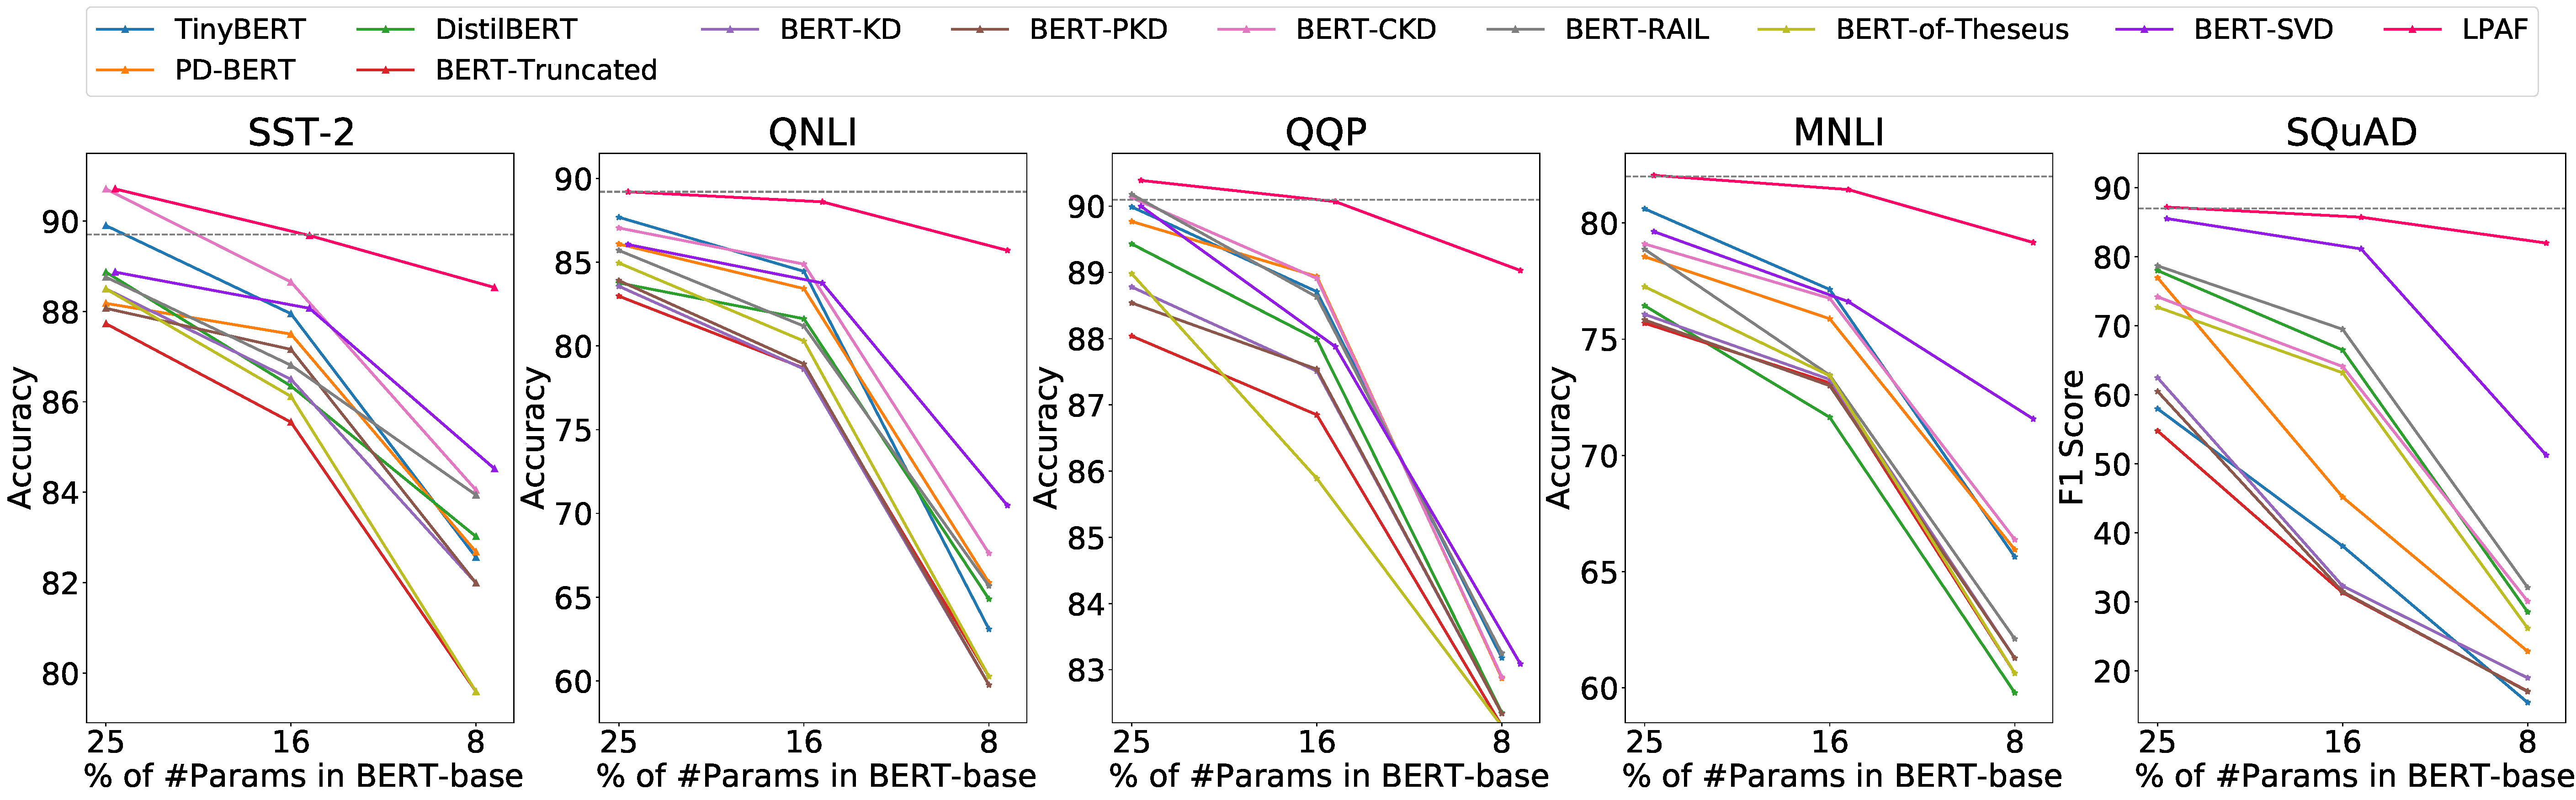
\includegraphics{./figures/all.pdf}}
%	\caption{Experimental results~(average of 3 runs) of our proposed LPAF and all compared baselines. We use the horizontal gray line to indicate the performance of $T_{sparse}$ for reference purpose.} 
%\label{fig:all}
%\end{figure*}




\tabref{table:diffk} shows the results of LPAF with various preserved rank $k$. 
Compared to densely fine-tuned BERT, $T_{sparse}$ obtained by SMvP inevitably shows a slight performance drop 
on all tasks with an average sparsity of 86.3\%. Despite a large portion of parameters being pruned away, an unstructured pruning algorithm like SMvP does not result in an actual reduction in memory footprint and computational cost because the pruned weights are simply set to zero without being eliminated from the computation and storage. In contrast, LPAF exhibits up to 85\% and 82\% perceivable decrease of memory and computation respectively~(i.e., choosing $k=80$), meanwhile retaining task accuracy comparable to $T_{sparse}$. In summary, LPAF can achieve 
a 5.4x-12.3x reduction in model size and 4.6x-10.6x reduction in 
computation cost  while 
retaining 99\%-93\% of the performance of the original BERT.
%Comparing \tabref{table:diffk} with \tabref{table:pilot}, we can see that LPAF consistently outperforms SVD under every choice of $k$ by a large margin. The improvement is more evident under a high compression regime. For example, LPAF-40 outperforms SVD-40 by 15.2 percentage 
%points on QNLI and 5.9 points on QQP, respectively. Overall, LPAF shows much strong 
%compression performance than SVD, demonstrating the importance of a 
%low-rank structure for factorization.


\subsubsection{Comparisons with Baselines}
\tabref{table:all} summarizes the overall results. BERT$_{\text{Truncated}}$ performs the worst on all tasks. Among task-specific distillation methods, CKD shows the best overall performance thanks to its better initialization using PD-BERT and the use of a sophisticated distillation objective. Task-agnostic distillation methods generally outperform task-specific distillation methods except for CKD, showing that a pre-training compression stage is helpful when the compression ratio is high. SVD shows an obvious advantage over other baselines under a high compression ratio. This is because when the models are too shallow, i.e.,  less than 3 layers, the model capacity becomes insufficient. In contrast, SVD reduces model size at the matrix level while keeping the number of layers unchanged. Under all compression ratios, LPAF consistently gives the best results, verifying its general effectiveness. For extreme compression ratio, 
e.g., 8\%  on SST-2, LPAF shows a large advantage by retaining 96.2\% and 98.6\% accuracy of fine-tuned BERT and $T_{sparse}$. On the SQuAD dataset, LPAF shows up to 30.2 points improvement over SVD, showing its generality beyond classification tasks. Through controlled ablations, we can see that low-rank sparsity plays the most critical role to task accuracy, while sparsity-aware SVD and mixed-rank fine-tuning also yield consistent improvements by more accurate sparse matrix approximation and regularized training.




\subsection{Analysis}
\label{sec:analysis}

\begin{table}[t]
	\centering
	\scriptsize
	\begin{tabular}{|l|llll|}
		%		\toprule
		\hline
		&	\multicolumn{4}{c|}{$T_{sparse}$} \\
		%		\midrule
		\hline
		\multicolumn{1}{|l|}{$\tau$}           &0.1  &0.2  &0.3           &0.4                      \\
		\multicolumn{1}{|l|}{\% of Parameters}           & 30\% & 25\% & 16\%          & 10\%                     \\
		\multicolumn{1}{|l|}{Rank}               &545   &471   &349            &294                        \\
		\multicolumn{1}{|l|}{Accuracy}           & 90.9 & 90.3 & 89.1          & 88.2                     \\
		
		%		\midrule
		\hline
		\multicolumn{1}{|l|}{$k$=120}       &\textbf{90.1}  &89.5  &89.0           &88.6                      \\
		\multicolumn{1}{|l|}{$k$=100}        &88.8  &\textbf{89.5}  &88.4           &88.4                      \\
		\multicolumn{1}{|l|}{$k$=80}                  &87.2  &\textbf{89.3}  &88.2  &87.4                      \\
		\multicolumn{1}{|l|}{$k$=60}                  &87.1  &87.3  &88.0           &\textbf{88.2}             \\
		\multicolumn{1}{|l|}{$k$=40}                  &85.1  &85.3  &85.8           &\textbf{87.2}             \\
		%		\bottomrule
		\hline
	\end{tabular}
	\caption{Effect of different $T_{sparse}$ on SST-2.
	}
	\label{table:diffsparse}
\end{table}
\paragraph{Effect of different $T_{sparse}$} 
Recall that we choose the low-rank sparse model $T_{sparse}$ with at least 97\% of the fine-tuned BERT's performance. Here we experiment with different $T_{sparse}$ by altering threshold $\tau$ and examine its effect on the performance of LPAF \textit{without} sparsity-aware SVD and mixed-rank fine-tuning.
% \KZ{Why experiment with QNLI here while test with SST-2 for the next two subsections? Some people might be suspecting 
%something fishy.}
The results on SST-2 are summarized in \tabref{table:diffsparse}. As we increase $\tau$, $T_{sparse}$ becomes more sparse and its rank also monotonically decreases. We observe that for a fixed $k$, the performance of LPAF-$k$ turns out to resemble a unimodal distribution of the rank of $T_{sparse}$: as the rank gets too high, the increased approximation error overturns the benefit of improved accuracy; when the rank is too low, the drop of accuracy also overturns the benefit of decreased approximation error. Generally, the best performance of LPAF-$k$ for a larger $k$ is achieved at a higher rank of $T_{sparse}$ compared to that of a smaller $k$.
%\KZ{This suggests that LPAF should be used at a $k$ compatible with the $k$ of the $T_{sparse}$?}
% Please add the following required packages to your document preamble:
% \usepackage{multirow}


\begin{table}[t]
	\centering
	\scriptsize
	\begin{tabular}{|l|lllll|}
		%		\toprule
		\hline
		Weighting Strategy         &$k$=120  & $k$=100  & $k$=80   & $k$=60   & $k$=40   \\
		%		\midrule
		\hline
		- w/ $\bm{S}$    &\textbf{89.5}  & \textbf{89.4} & \textbf{88.8} & \textbf{88.4} & \textbf{87.9} \\
		- w/ $\bm{M}$   &89.1   & 88.9 & 88.5 & 88.3 & 87.4 \\
		- w/o $\bm{S}$ or $\bm{M}$ &88.8 & 88.7 & 88.0 & 87.4 & 87.1 \\
		%		\bottomrule
		\hline
	\end{tabular}
	\caption{Ablation study of weighting strategies for SVD on SST-2 with vanilla fine-tuning.}
	\label{table:diffsvd}
\end{table}

\paragraph{Effectiveness of sparsity-aware SVD}
In our sparsity-aware SVD, the reconstruction error of each parameter $\bm{W}_{i,j}$ is weighted by its importance score $\bm{S}_{ij}$. To examine its effectiveness in factorizing sparse matrix, we experiment with two variants on SST-2 dataset: (1) $\bm{S}$ is replaced by coarse-grained binary score $\bm{M}$; (2) non-weighted vanilla SVD. \tabref{table:diffsvd} shows that weighting by importance score yields the best results under all $k$, and a simple binary weighting strategy using $\bm{M}$ also brings improvement compared to vanilla SVD. This means that our sparsity-aware SVD is still applicable even when $\bm{S}$ is unavailable.


As stated in \secref{sec:sasvd}, we expect sparsity-aware SVD to retain more task performance from $T_{sparse}$ compared to vanilla SVD. We verify this by comparing their performances before fine-tuning. 
\figref{fig:init} shows that by informing the matrix factorization process with sparsity, 
more task performance can be retained at the beginning. 
Also, weighting by importance score gives slightly better initial performance due to 
its finer granularity.
\begin{figure}[h]
	\centering
	\scalebox{0.260}{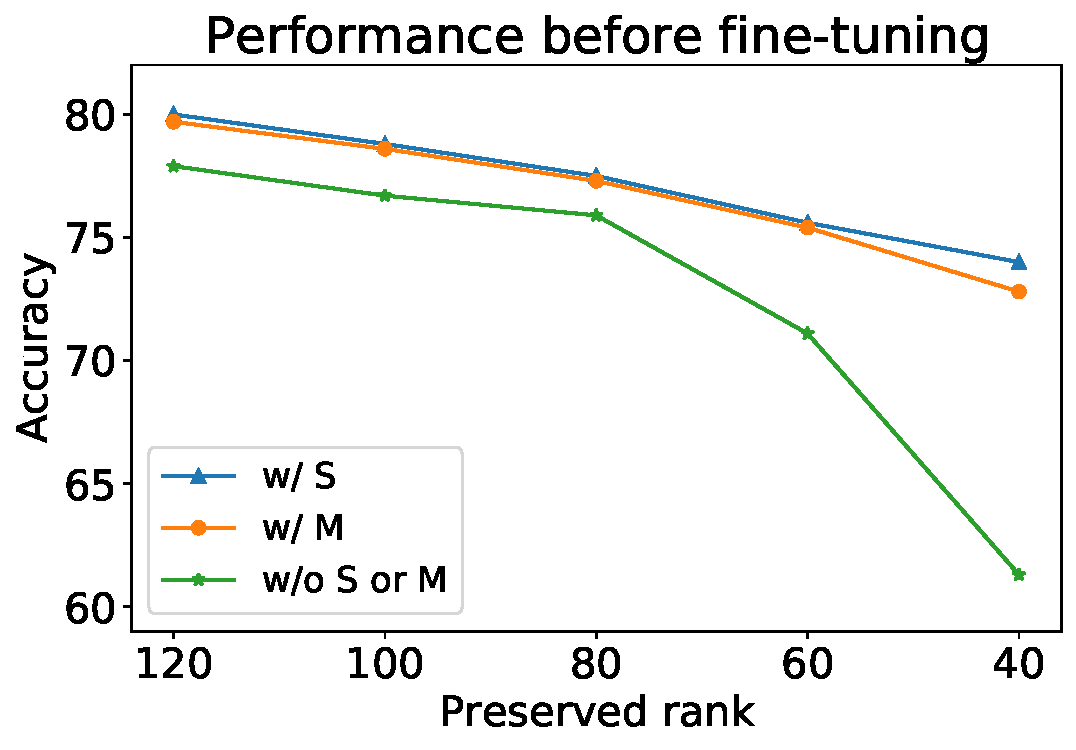
\includegraphics{./figures/init.pdf}}
	\caption{Performance of $T_{factorized}$ on SST-2 with different factorization methods before fine-tuning~(step-3).}
	\label{fig:init}
\end{figure}

\paragraph{Effectiveness of mixed-rank fine-tuning} In \tabref{table:wwomixedrank}, we examine the effectiveness of mixed-rank fine-tuning by ablation study.  Results show that mixed-ranking fine-tuning consistently brings improvement over standard fine-tuning under all choices of $k$. Adding the consistency objective $\mathcal{L}_{c}$  stabilizes training and leads to further improvement. 
\begin{table}[th]
	\centering
	\scriptsize
	\begin{tabular}{|l|lllll|}
%		\toprule
\hline
		Fine-tuning Method & $k$=120 & $k$=100 & $k$=80 &$k$=60 & $k$=40 \\
%		\midrule
		\hline
		mixed-rank      & \textbf{90.7}  & \textbf{90.3}  & \textbf{89.7} &\textbf{89.0}  & \textbf{88.5} \\
		- w/o $\mathcal{L}_{c}$    &89.8 &89.6   &89.1  &88.5 &88.1  \\
%		\midrule
\hline
		vanilla  & 89.5  & 89.4  &88.8  &88.4 & 87.9	 \\
%		\bottomrule
\hline
	\end{tabular}
	\caption{Ablation of mixed-rank fine-tuning on SST-2.}
	\label{table:wwomixedrank}
\end{table}

We also study the effect of using different values of $p_{init}$ on the performance of mixed-rank fine-tuning. From \tabref{table:diffp} we can see that: (1) for $T_{factorized}$ with smaller $k$, it prefers a relatively large $p_{init}$ because its model capacity is largely reduced and it can benefit more from mixed-ranking fine-tuning to improve generalization; (2) for $T_{factorized}$ with larger $k$, a smaller $p_{init}$ is more favorable because its higher capacity makes it less likely to converge into bad local minimum; (3) setting $p_{init}$ to zero makes our method loses regularization effect brought by gradient-level interaction between factorized sub-matrices and original sparse matrix, thus degenerating performance under all compression ratios.
\begin{table}[th]
	\centering
	\scriptsize
	\begin{tabular}{|cl|lllll|}
%		\toprule
\hline
		&     & $k$=120 & $k$=100 & $k$=80 & $k$=60 & $k$=40   \\
%		\midrule
\hline
		\multirow{3}{*}{$p_{init}$} & 0.7 & 90.2  & 89.8  & \textbf{89.7} & \textbf{89.0} & \textbf{88.5} \\
		& 0.5 & 90.5  & \textbf{90.3}  & 89.5 & 88.8 & 88.3 \\
		& 0.3 & \textbf{90.7}  & 89.6  & 89.0 & 88.5 & 88.1 \\
		& 0.0     & 90.0  & 89.6  & 89.3 & 88.5 & 87.7 \\
%		\bottomrule
\hline
	\end{tabular}
	\caption{Ablation study on different $p_{init}$ on SST-2.
		%	\KZ{If you reorg the $p_{init}$ in ascending order, you will see the bolded numbers organized in
		%a diagonal pattern similar to Table 5. Does that suggest anything?}
	}
	\label{table:diffp}
\end{table}


\subsection{Applicability to Other PLMs}
LPAF is model architecture-agnostic in that it operates purely on the 
matrix level throughout all stages. It is straightforward to apply LPAF to other pre-trained language models beyond BERT. To this end, we apply  LPAF to compress an already compact 12-layer and 384 hidden-dimension MiniLMv2~\cite{minilm} with 21.5M parameters into even smaller ones with \{33\%, 25\%\} of original parameters. The results are shown in \tabref{table:roberta}. For LPAF, we observe a similar low-rank phenomenon~(281 on average) in the sparse model, demonstrating the general low-rank sparse pattern induced by first-order weights pruning. The final model compressed by LPAF consistently outperforms those compressed by truncation, SVD$_{\text{Ft}}$, and the strong distillation method CKD, which confirms its general applicability.
\begin{table}[h]
	\centering
	\scriptsize
	\begin{tabular}{|c|ccc|}
		%		\toprule
		\hline
		Task & SQuAD v1.1   & QNLI     & MNLI-m/mm         \\
		%		\midrule
		\hline
		\% of \#Parameters &33\%  ~~25\%            &~33\%  ~~25\%             &~33\%  ~~~~~~~~25\%          \\
		%		\midrule
		\hline
		Truncated       & 82.4 ~76.3          & 86.5~ 83.2          & 79.8/80.4~ 75.3/75.9         \\
		CKD       & 83.7 ~77.8          & 87.2~ 83.3          & 80.0/80.6~ 75.4/76.0         \\
		
		%		\midrule
		\hline
		SVD$_{\text{Ft}}$           & 83.1 ~78.2          & 86.0~ 83.5          & 80.3/81.0~ 77.5/78.6         \\
		LPAF~(ours)                  &\textbf{85.4} ~\textbf{83.9}          & \textbf{88.6}~ \textbf{87.8}          & \textbf{82.4/83.1}~ \textbf{81.5/82.3}           \\
		%		\bottomrule
		\hline
	\end{tabular}
	\caption{Results~(average of 3 runs) of compressing MiniLMv2 into 33\%/25\% of original parameters on representative natural language understanding tasks.}
	\label{table:roberta}
\end{table}



